\section{Layer~10 – Global Meta‑Ontological Evaluation}
\label{sec:layer10}

% ----- SUPERKRACHT -----
\begin{tcolorbox}[colback=blue!5, colframe=blue!60, title=\textbf{Superpower: The Editor}]
\begin{center}
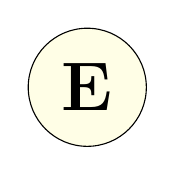
\begin{tikzpicture}
  \node[draw, circle, fill=yellow!10, minimum size=1.5cm, font=\bfseries\Huge] {E};
\end{tikzpicture}
\textit{“Do my ideas fit together?”}
\end{center}
\end{tcolorbox}

New concepts are fun, but what if they contradict each other?  Layer~10
acts as an \textbf{editor‑in‑chief}: it checks whether all categories,
rules, and predictions form a coherent whole.

\begin{tcolorbox}[colback=yellow!5, colframe=yellow!80, title=Real‑life analogy]
An encyclopaedia has an editorial team that checks whether the article
about “dog” doesn’t claim that dogs can fly, while the article about
“wings” says dogs have no wings.  Layer~10 performs that check for
Pixel’s entire knowledge base.
\end{tcolorbox}

\textbf{The coherence score.}
Pixel computes a \textbf{coherence score} – a report grade that
indicates how consistent its world‑view is.  If the score drops,
Pixel knows it needs to revise a few ideas.  This makes it not only
smarter, but also \emph{more honest}: it cannot simply hold on to a
contradictory thought.